\section*{Información General para la evaluación}
Di lunedì seminarios fino a fine marzo...
I seminari sono parte del$ 25\%$ della observación
Da marzo iniziano le prácticas, che sono un altro $25\%$
$30\%$ è una prova scritta
$20\%$ è una prova orale 

\chapter{Calidad}

\section{¿Qué entendemos por ``sistema de información''}

\begin{definition}[Sistema de información]
   Conjunto único de hardware, software, bases de datos,
   telecomunicaciones, personas y procedimientos configurado
   para recolectar, manipular, almacenar y procesar datos para
   convertirlos en información
\end{definition}

Entonces un sistema de información necesita de una \textbf{entrada} de datos, un \textbf{procesamiento} de los mismos y una \textbf{salida} de información.

\section{Calidad}
\begin{definition}[Calidad - 1] 
   La calidad para Pressman (1998) es el \textit{cumplimiento} con:
   \begin{itemize}
      \item los requerimientos funcionales y de rendimiento explícitamente establecidos,
      \item los estándares de desarrollo explícitamente documentados
      \item con las características implícitas que se esperan de todo
      software desarrollado profesionalmente.
   \end{itemize}
\end{definition}

\begin{definition}[Calidad - 2]
   Según las standards ISO e IEEE la calidad es
   El grado con el que un sistema, componente o proceso
   cumple con los requisitos especificados y las necesidades o
   expectativas del cliente o usuario.
\end{definition}

\begin{definition}[Calidad - 3]
   Según la ISO 91260, la calidad es el conjunto de propiedades
La totalidad de características de un producto de software
que tienen como habilidad, satisfacer necesidades explícitas o
implícitas.
\end{definition}

\subsection{Modelos de Calidad}
Los modelos de calidad son herramientas que permiten evaluar la calidad de un producto o servicio. Ellos apuntar a identificar características estándar relacionadas con la
calidad del software a través de atributos de calidad.
{Atributos de calidad incluyen:\ns
\begin{itemize}
   \item Adeguación Funcional
   \item Seguridad
   \item Fiabilidad (reliability)
   \item Usabilidad
   \item Eficiencia
   \item Mantenibilidad
   \begin{itemize}
      \item Reparabilidad
      \item Adaptabilidad
      \item Portabilidad
   \end{itemize}
   En relación con Mantenibilidad, el OPEN/CLOSED principle dice que \ul{un software debe estar abierto para extensión pero cerrado para modificación}. 
   \item Compatibilidad
\end{itemize}
\note{Estos atributos pueden cambiar según los modelos}
}

En general los atributos pueden ser esternos o internos. Los primeros derivados de la relación entre el entorno y el sistema (para ello, el proceso o el sistema debe ejecutarse), e.g. reliability, robustness, usability. Los segundos derivados directamente de la descripción del producto o del proceso.

\subsection{Métricas}
{Es necesario desarollar métricas de calidad, que deben ser:\ns
\begin{itemize}
   \item Simples y faciles da usar
   \item Empírica e intuitivas
   \item Consistente y objectivas
\end{itemize}}

Por ejemplo, centrémonos en la mantenibilidad. Podemos medirla con las siguientes métricas:
\begin{itemize}
   \item Aclopamiento
   \item Cohesión
   \item Complejidad Ciclomática de McCabe
   \item Código Chum
   \item Code Coverage
   \item Código Muerto
   \item Duplicación de Código
   \item 
\end{itemize}


\section{Requisitos}
Los requisitos son fundamentales en el software, y pueden ser utilizados para medir la calidad de este. 
Pero es importante notar que es necesario poder verificar si los requisitos están satisfechos con la implementación.
Además, necesitamos también algunos controles sobre los requisitos, come complejidad, consistencia, completitud, corrección, claridad, verificabilidad, rastreabilidad, prioridad, viabilidad, flexibilidad, no ambigüedad, no redundancia, no contradicción, no vaguedad, no sobre-especificación, no sub-especificación.
% TODO verifica requisitos controles

Requisitos no funcionales son más fáciles de verificar que los funcionales, porque son más objetivos.
\begin{definition}
   [Requisito no funcional verificable]
   Una frase que incluye alguna medida que puede ser objetivamente probada.
\end{definition}

Matrices de trazabilidad son herramientas que permiten verificar la trazabilidad de los requisitos.
Hay muchas matrices en las slides, algunas relacionan requisitos con casos de uso, otros con pruebas, otros con componentes del sistema.

\framedt{Ejercicio 1 / Analisis Requisitos}{
   Javier dice cosas correctas. Aparte de las cosas que mencionó, se puede ver cómo no hay muchos numeros en los requisitos; el documento dices que es necesario hacer backups, pero, ¿cuantós backups? ¿con qué frecuencia? ¿con qué software?.
}

\section{Gestión de la Calidad}
La calidad del proceso contribuye a la calidad del producto, y la calidad del producto contribuye a la calidad en uso.
\note{
   \begin{itemize}
      \item \textbf{Producto}: entregado al cliente
      \item \textbf{Proceso}: conjunto de actividades que se realizan para producir un producto
   \end{itemize}
}



Hay algunos pasos importantes en la gestión de la calidad:
\begin{itemize}
   \item Preparación y utilización de recursos
   \begin{itemize}
      \item Humanos
      \item Económicos
      \item Infraestructura
      \item Conocimientos y experencia
   \end{itemize}
   \item Procesos
   \begin{itemize}
      \item Estratégicos
      \item Operativos
      \item Soporte
   \end{itemize}
   \item Políticas de trabajo\\
   Una política de trabajo de calidad es una manifestación que realiza una empresa acerca de cómo actúa y cuáles son las pautas o reglas que establecen en el día a día para trabajar que le lleven a mejorar continuamente y hacer las cosas bien a la primera.

   Una parte crítica de la política de calidad es detectar y analizar los problemas en una empresa y los resultados no alcanzados
   \item Objetivos\\
   ``Conseguir una productividad del 100\% de los desarrolladores'' o ``Aumentar la satisfacción de los cliente'' son objetivos mal planteados.

\end{itemize}

\subsection{ISO 9001}
La ISO 9001 es una norma internacional que especifica los requisitos para un sistema de gestión de la calidad (SGC). Las organizaciones utilizan la norma para demostrar la capacidad para proporcionar productos y servicios que cumplen con los requisitos del cliente y los reglamentarios aplicables.
El principal objetivo de la ISO 9001:2015 es lograr que una compañía consiga la satisfacción del cliente mediante el establecimiento de procesos de mejora continuada dentro de la misma.

Propone también un metodo de \textbf{mejora continua}, el PDCA (Plan, Do, Check, Act).

\subsubsection{Quality control and assurance}
\begin{itemize}
   \item \textbf{Quality Control}: A part of quality management focused on fulfilling quality
   requirements\\
   Parte de la gestión de calidad de software que comprueba que el proyecto sigue sus estándares, procesos y procedimientos, y que el proyecto produce los productos (entregables) internos y externos requeridos.
   \item \textbf{Quality Assurance}: A part of quality management focused on providing confidence that quality requirements will be fulfilled\\
   Parte de la gestión de calidad de software que asegura que los estándares, procesos y procedimientos son apropiados para el proyecto y se han implementado correctamente.
\end{itemize}

\begin{itemize}
	\item los \textit{procesos} incluyen todas las actividades involucradas en el
diseño, codificación, pruebas y mantenimiento;
	\item los \textit{productos} incluyen software, datos asociados,
documentación, y toda la documentación para soporte y
reportes.
\end{itemize}

Los ingenieros del software realizan el trabajo técnico.
En cambio, un grupo de SQA (Software Quality Assurance) se responsabiliza en la planificación de aseguramiento de la calidad, supervisión, mantenimiento de registros, análisis e informes.\\
El principal propósito del control de calidad es asegurar que el producto satisface los requisitos mediante \textbf{pruebas} y \textbf{revisiones} de los requisitos funcionales y no funcionales.

\subsubsection{SPI - Software Process Improvement}

\begin{figure}[htbp]
   \centering
   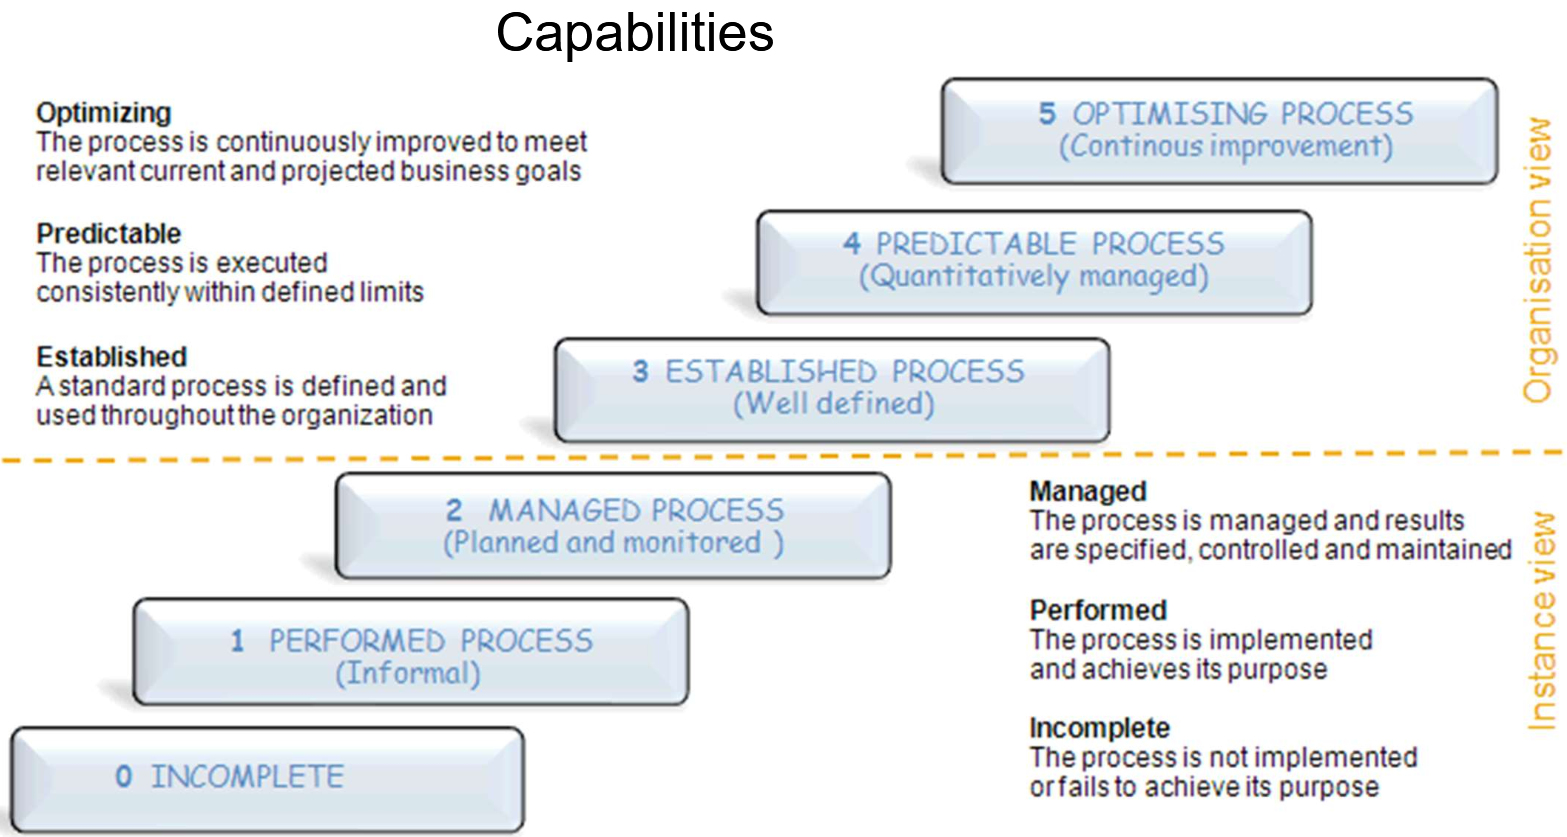
\includegraphics{images/01/spice.png}
   \caption{Spice Model for Process Improvement}
   \label{fig:01/spice}
\end{figure}

\begin{paracol}{2}
   Modelos de Madurez establecen marcos de referencia que evalúan la capacidad de una organización para desarrollar productos o servicios de calidad de manera consistente y predecible; van a evalúar la madurez de los procesos de desarrollo de software o sistemas.
   
   \switchcolumn

   \begin{figure}[htbp]
      \centering
      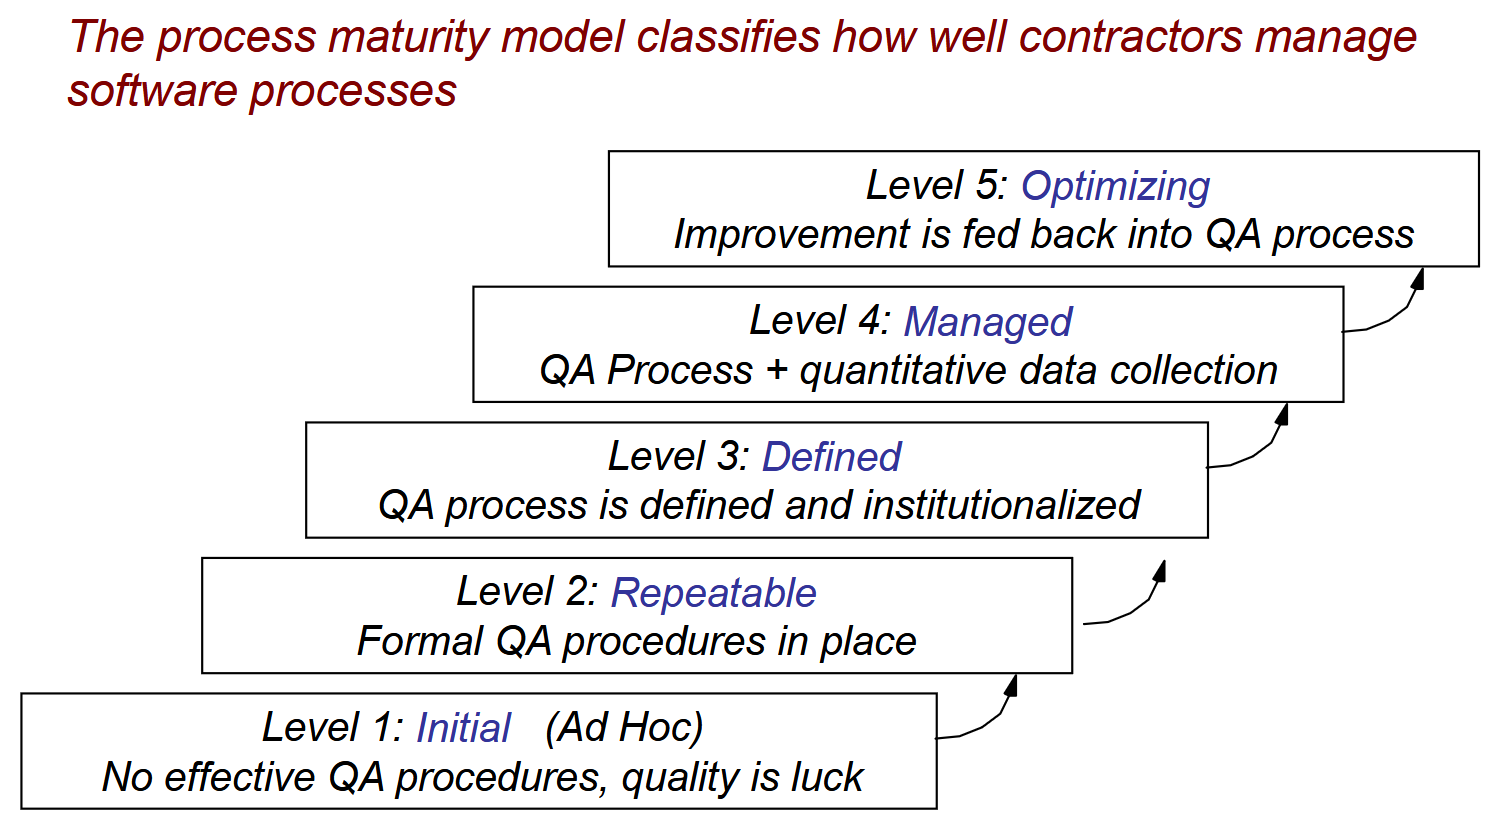
\includegraphics{images/01/madurez.png}
      \caption{Capability Maturity CMMI}
      \label{fig:01/madurez}
   \end{figure}

\end{paracol}

\framedt{Complaints about Models}{
	\begin{itemize}
		\item No siempre se ven como tan relevantes y actuales por los
		      ingenieros del software
		\item Pueden conllevar mucha burocracia
		\item Pueden requerir trabajo manual tedioso si no tienen
		      herramientas software de soporte
	\end{itemize}
	Entonces, \textit{to effectively apply standards, limit overhead!}
}

\subsection{Coste de la calidad}
\begin{equation}
   \text{Coste de la calidad} = \text{Coste de conformidad} + \text{Coste de no conformidad}
\end{equation}

\begin{definition}
	[Coste de conformidad]
	costes de las actividades para:
	\begin{itemize}
		\item Valoración/Estimación: detección de defectos (testeo)
		\item Prevención: de errores (aseguramiento de calidad, etc)
	\end{itemize}
\end{definition}


\begin{definition}
   [Coste de no conformidad]
   costes de las actividades para:
   \begin{itemize}
      \item Corrección: de defectos (reparación de errores)
      \item Fallos: en el producto (retrabajo, etc)
      \item Pérdida de clientes
      \item Costes de juicios
      \item etc.
   \end{itemize}
\end{definition}

\begin{figure}[htbp]
   \centering
   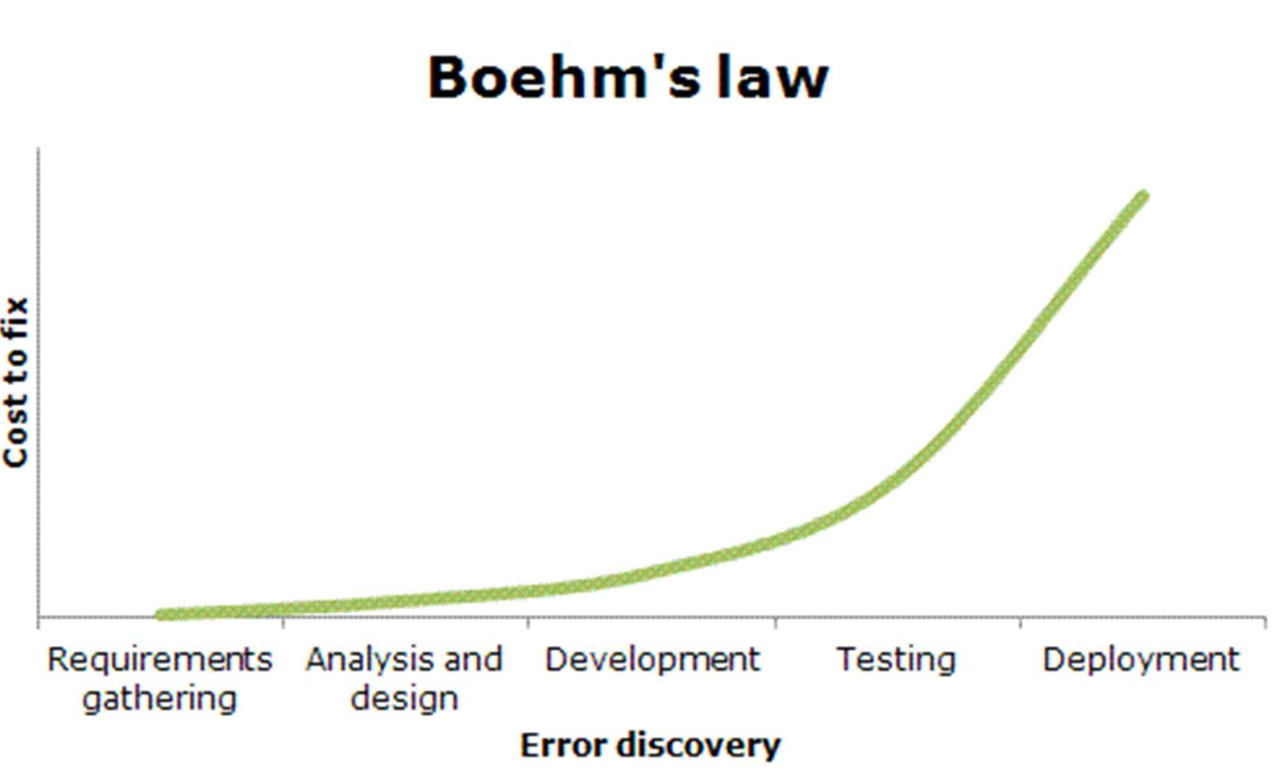
\includegraphics{images/01/boehm.png}
   \caption{Según Boehm, el coste de corregir un error aumenta exponencialmente con el tiempo. Entonces, el \textbf{testing} es un momento crítico en el desarrollo de software, porque permite de encontrar errores antes de que el coste de corregirlos sea más alto.}
   \label{fig:01/boehm}
\end{figure}